%\section{Mechanical properties}
%\label{sec:m_properties}

Constitutive equations (i.e. constitutive relations, material laws) are relations between measures of deformation (e.g. strain tensor) and internal force density functions (stress tensor) resulting from the action of external forces. Usually, they are not laws of nature but represent mathematical models intended to characterize the typical material behavior based on physically reasonable assumptions (particularly consistent with the thermodynamic balance relations) and mathematically correct approaches.

\subsection{Effective stress principle}
\label{sec:effstress}

Following the statements given in section~\ref{sec:momentum_balance} the total Cauchy's stress tensor in porous media is decomposed in partial stresses referring to the participating phases (note the sign convention of positive fluid phase pressure $p^{\gamma}$, but negative compressive normal stress for the solid phase).
\begin{equation}
\miu{\sigma}{}{}\,=\,(1-n)\,\mio{\sigma}{s}{}\,-\,n
\left(\sum\limits_{\gamma}S^{\gamma}\,p^{\gamma}\right)\mathbf{I}
\label{eq:totalstress}
\end{equation}
Considering the effective stress principle, relation (\ref{eq:totalstress}) can be modified defining the effective solid stress $\mib{\sigma}{eff}{s}{}$ as well as the overall fluid pressure $p^{\gamma}$
\begin{eqnarray}
\miu{\sigma}{}{} & = & 
(1-n)\left[
\mio{\sigma}{s}{}\,+\,\left(\sum\limits_{\gamma}S^{\gamma}\,p^{\gamma}\right)\mathbf{I}
\right]
\,-\,\left(\sum\limits_{\gamma}S^{\gamma}\,p^{\gamma}\right)\mathbf{I} \nonumber \\
 & = &
\miu{\sigma}{\mathrm{eff}}{}{}
\,-\,\left(\sum\limits_{\gamma}S^{\gamma}\,p^{\gamma}\right)\mathbf{I}
\label{eq:effect_stress}
\end{eqnarray}
The effective solid stress is the total solid stress reduced by the excess pore liquid pressure, but referred to the domain of the overall porous medium. Consequently, its absolute value is lower than the intrinsic stress of the solid skeleton. Constitutive relations for the solid phase of porous media combine the solid skeleton deformation (in terms of the strain tensor) with the effective solid stress. Selected models are presented in the next paragraphs. As they are equally valid for single-phase solid materials as well as for the solid phase of porous media, the special notation of the effective stress tensor will be omitted without loss of generality.

Based on the stress decomposition (\ref{eq:effect_stress}), the equilibrium condition for the porous medium becomes
\begin{equation}
\rho \mio{g}{}{}
+
\,\nabla\,\cdot\,\miu{\sigma}{\mathrm{eff}}{}{}\,
-
\left(\sum\limits_{\gamma}S^{\gamma}\,p^{\gamma}\right)\mathbf{I}
=
\,\mathbf{0}
\label{eq:equi_mod}
\end{equation}

%---
\subsection{Material classes}
\label{sec:matclass}

Usually laboratory tests are performed on specimens to investigate the mechanical behavior. Within this context, similar stress-strain curves can be caused by different physical effects, e.g. a nonlinear stress-strain curve does not necessarily suggest inelastic material behavior. For the sake of clarity, it is possible to introduce a classification of materials based on some essential distinctly identifiable material phenomena. For instance, comparatively simple experiments can be performed to investigate if the stress-strain curves are rate-dependent, and if hysteresis phenomena occur indicating dissipative effects.

\begin{figure}[htb!]
\begin{center}
\footnotesize
\includegraphics[width=0.95\textwidth]{figures/matbehav_el_elpl.eps}
\caption{Experimentally observed rate-independent solid material behavior. Cyclic uniaxial stress-strain curves \cite{Haupt:2002}: elasticity (left) and elastoplasticity (right)}
\label{fig:matbehav_el_elpl}
\end{center}
\end{figure}
\begin{figure}[htb!]
\begin{center}
\footnotesize
\includegraphics[width=0.95\textwidth]{figures/matbehav_vel_vpl.eps}
\caption{Experimentally observed rate-dependent solid material behavior. Cyclic uniaxial stress-strain curves \cite{Haupt:2002}: viscoelasticity (left) and viscoplasticity (right)}
\label{fig:matbehav_vel_vpl}
\end{center}
\end{figure}

\newpage

Based on these assumptions the observable material behavior can be divided into four different basic classes:
\begin{itemize}
\item rate-independent without hysteresis,
\item rate-independent with hysteresis,
\item rate-dependent without hysteresis, and
\item rate-dependent with hysteresis.
\end{itemize}
Figs.~\ref{fig:matbehav_el_elpl} and \ref{fig:matbehav_vel_vpl} schematically show typical cyclic stress-strain curves for these material classes. The equlibrium curves, presented in Figs.~\ref{fig:matbehav_vel_vpl} can be observed as a result of relaxation experiments.

According to the experimental observations, there are four classes of mathematical models matching the material classes defined above:
\begin{itemize}
\item the theory of elasticity describes rate-independent material behavior without hysteresis,
\item the theory of (elasto)plasticity describes rate-independent material behavior with hysteresis,
\item the theory of viscoelasticity describes rate-dependent material behavior without hysteresis, and
\item the theory of viscoplasticity describes rate-dependent material behavior with hysteresis.
\end{itemize}

Physically significant constitutive relations in the uniaxial case can be defined for the four classes of material theories based on so-called rheological models. These complex models consist of a simple networks of individual rheological elements (cf. Fig.~\ref{fig:rheomod_elem}), like
\begin{itemize}
\item elastic springs, which correspond to the linear stress-strain relation
\begin{equation}
\sigma\,=\,k\,\varepsilon
\end{equation}
with the spring constant $k$ representing the proportionality factor,  
\item viscous dashpots, which represent Newtonian viscous substances, and obey a linear relation between stress and strain rate
\begin{equation}
\sigma\,=\,\eta\,\mathop{\varepsilon}\limits^{\miu{.}{}{}}
\end{equation}
with the proportionality factor $\eta$ characterizing the viscosity, and
\item Coulomb friction elements, resisiting any motion until a threshold stress $\sigma^{\star}$ is reached, whereas behind the threshold irreversible deformations occur
\begin{equation}
\varepsilon\,=\,
\left\{
\begin{array}{ll}
0,              & \qquad\mbox{if}\quad\sigma\,<\,\sigma^{\star}  \\[1.5ex]
\varepsilon(t), & \qquad\mbox{if}\quad\sigma\,\geq\,\sigma^{\star}
\end{array}
\right.
\end{equation}
\end{itemize}

\newpage

\begin{figure}[htb!]
\begin{center}
\footnotesize
\includegraphics[width=0.95\textwidth]{figures/rheomod_elements.eps}
\caption{Mathematical modeling of solid material behavior. Basic individual elements of rheological models \cite{JCZ:2007}: spring element (left), dashpot element (middle) and frictional element (right)}
\label{fig:rheomod_elem}
\end{center}
\end{figure}

Differential equations, which are defined based on an appropriate composition of rheological models are only in a few special cases suitable to describe material response to external loading observed in reality. They can rather serve for marking the physical significance of mathematical models within the context of material theories. In Figs.~\ref{fig:rheomod_el_elpl} and \ref{fig:rheomod_vel_vpl} typical rheological models are presented, which characterize the material behavior of the four material classes defined above.

\begin{figure}[htb!]
\begin{center}
\footnotesize
\includegraphics[width=0.95\textwidth]{figures/rheomod_el_elpl.eps}
\caption{Mathematical modeling of rate-independent solid material behavior. Cyclic uniaxial stress-strain curves \cite{Haupt:2002}: elasticity (spring element -- left) and elastoplasticity (spring and frictional elements -- right)}
\label{fig:rheomod_el_elpl}
\end{center}
\end{figure}

\begin{figure}[htb!]
\begin{center}
\footnotesize
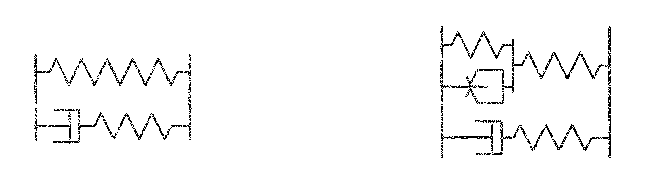
\includegraphics[width=0.95\textwidth]{figures/rheomod_vel_vpl.eps}
\caption{Mathematical modeling of rate-dependent solid material behavior. Cyclic uniaxial stress-strain curves \cite{Haupt:2002}: viscoelasticity (spring and dashpot elements -- left) and viscoplasticity (spring, dashpot, and frictional elements -- right)}
\label{fig:rheomod_vel_vpl}
\end{center}
\end{figure}

In Tab.~\ref{tab:matclass} some typical technical as well as natural (including geological) materials are assigned to the generalized material classes considering their material behavior, which can be observed for characteristic application cases. Generally, the classification of the material behavior depends on the real loading regime (e.g. small or large strains), environmental conditions (e.g. temperature), and the time scale of the physical processes under consideration. Changing one or more of these conditions one and the same material can demonstrate different mechanical behavior. Basically, no materials are actually purely elastic over a wide range of stresses, temperature, and time. Otherwise, developing and using complex constitutive models, which include all observable phenomena is not advisable for practical reasons. Constitutive relations, rather, should represent idealized and simplified models according to the most dominating conditions appearing in the practical applications under consideration.

\renewcommand{\arraystretch}{1.25}
\begin{table}[htb!]
\caption{Generalized classes of solid material behavior, and selected, typical representatives}
\label{tab:matclass}
\begin{center}
%\begin{tabular}{|l||l|l|}
\begin{tabular}{|p{0.18\textwidth}||p{0.37\textwidth}|p{0.33\textwidth}|}
\hline
Material class & Technical/natural material & Geomaterial \\
\hline\hline
elasticity & metals at small strains, & igneous rocks                 \\
           & ceramics,                & (e.g. granite),               \\
           & bone,                    & hard sedimentary rocks        \\
           & most other materials at small strains & (e.g. sandstone) \\
\hline
elastoplasticity & metals at large strains & most soils,                        \\
                 &                         & soft sedimentary rocks (e.g. tuff) \\
\hline
viscoelasticity & rubber,                 & rock salt (halite) \\
                & glass,                  &                    \\
                & soft biological tissues &                    \\
\hline
viscoplasticity & polymers (plastics),       & clay soils, \\
                & wood,                      & clay stone  \\
                & bitumen,                   &             \\
                & metals at high temperature &             \\
\hline
\end{tabular}
\end{center}
\end{table}
\renewcommand{\arraystretch}{1.00}
%
\hfill
%-------------------------------------------------------------------------
\newpage
\subsection{Elasticity}
\label{sec:elasticity}

In a micromechanical point of view, elasticity is predominantly caused by the evolution of interatomic forces in response to the impact of
external forces. It can be observed for crystalline substances (where the atoms are established in regular structures) as well as for
amorphous materials (where the atoms compose irregular structures), and is characterized by reversibility of the deformation processes and
the absence of any hysteresis. Furthermore, it is assumed that the current stress state is uniquely defined by the current strain state,
and does not depend on the strain history. Consequently, within the context of the constitutive model, the stress tensor is a function of
the strain tensor, but it does not depend on the strain rate. 

The isothermal isotropic linear elastic material model 
\begin{equation}
\miu{\sigma}{}{}\,=\,2\mu\,\miu{\varepsilon}{}{}\,+\,\lambda\,\mathrm{tr}(\miu{\varepsilon}{}{})\,\mathbf{I}
\label{eq:hooke_isotherm}
\end{equation}
known as generalized Hooke's law is the simplest of all constititive models for solid material behavior. Instead of the so-called
Lam{\'{e}} constants $\mu$ and $\lambda$, Hooke's law is often represented in terms of other material parameters like the Young's modulus
(i.e. elastic modulus, coefficient of elasticity, modulus of elasticity et al.) $E$, the Poisson's ratio $\nu$, the shear modulus $G$, and
the bulk modulus $K$. Some useful relations between these parameters are as follows:
\begin{eqnarray*}
E & = & \mu\,\ttfrac{2\mu+3\lambda}{\mu+\lambda},\qquad
\nu\,=\,\ttfrac{\lambda}{2(\mu+\lambda)} \\[2.0ex]
\mu & = & \ttfrac{E}{2(1+\nu)},\qquad
\lambda\,=\,\ttfrac{\nu E}{(1+\nu)(1-2\nu)} \\[2.0ex]
G & = & \ttfrac{E}{2(1+\nu)}\,=\,\mu \\[2.0ex]
K & = & \ttfrac{E}{3(1-2\nu)}\,=\,\ttfrac{(\mu+\lambda)(2\mu+3\lambda)}{3}
\end{eqnarray*}
Thus, the coefficients of the consistent material matrix $d\miu{\sigma}{}{}/d\miu{\varepsilon}{}{}$, which is required for the numerical
simulation of mechanical material behavior can be representeed in case of linear elasticity straightforward.
\begin{equation}
\fourtens{C}
\equiv
{C}_{ijkl}\,=\,\frac{d\sigma_{ij}}{d\varepsilon_{kl}}\,=\,2\mu\,\delta_{ik}\,\delta_{jl}\,+\,\lambda\,\delta_{ij}\,\delta_{kl}
\end{equation}

If a coupling of mechanical and thermal processes occur (non-isothermal mechanical processes), in addition to the strain caused by the
impact of external forces a volumetric thermal strain can be observed, which usually is linearly related to
the temperature difference.
\begin{equation}
\miu{\varepsilon}{\mathrm{th}}{}\,=\,\alpha_T\,(T-T_0)\,\mathbf{I}
\end{equation}
Here, $\alpha_T$ denotes the linear thermal expansion coefficient, and $T_0$ the initial temperature. In small strain solid mechanics it is
common practice to consider additive decompositions of the overall strain tensor into several constitutive parts according to the observed
physical phenomena. Considering thermoelastic material behavior, the overall strain tensor consists of an elastic part and a thermal part.
\begin{equation}
\miu{\varepsilon}{}{}\,=\,\miu{\varepsilon}{\mathrm{el}}{}\,+\,\miu{\varepsilon}{\mathrm{th}}{}
\end{equation}
As Hooke's law (\ref{eq:hooke_isotherm}) has to be perceived as a constitutive model, which assigns the local stress state to local elastic
strains, a non-isothermal generalization can be defined easily. 
\begin{equation}
\miu{\sigma}{}{}\,=\,2\mu\,\miu{\varepsilon}{\mathrm{el}}{}\,+\,\lambda\,\mathrm{tr}(\miu{\varepsilon}{\mathrm{el}}{})\,\mathbf{I}
                \,=\,2\mu\,\miu{\varepsilon}{}{}\,+\,\lambda\,\mathrm{tr}(\miu{\varepsilon}{}{})\,\mathbf{I}
                \,-\,(2\mu+3\lambda)\,\miu{\varepsilon}{\mathrm{th}}{}
\label{eq:hooke_nonisotherm}
\end{equation}
A conclusion drawn from Hooke's law of linear elasticity is the specific representation of the equilibrium condition for a thermo-poro-elastic porous medium in case of small strains.
\begin{equation}
\nabla\,\cdot\,
\left(
\miu{\sigma}{\mathrm{eff}}{}{}(\miu{\varepsilon}{}{})\,-\,
\left(\sum\limits_{\gamma}S^{\gamma}\,p^{\gamma}\right)\mathbf{I}\,-\,
\frac{2\mu+3\lambda}{3}\,\alpha_T\,(T-T_0)\,\mathbf{I}
\right)
\,=\,\rho\,\mio{g}{}{}
\label{eq:equi_thermo_poro_elast}
\end{equation}

Although no materials are actually linearly elastic over a wide range of stresses, elastic constitutive models are often quite useful and
accurate in many practical applications, e.g. in rock mechanics. The elastic material parameters given in Tab.~\ref{tab:rockelastpar} for 
selected soils and rocks show the large variation of material parameters, which is typical for geomaterials. 

\renewcommand{\arraystretch}{1.25}
\begin{table}[htb!]
\caption{Elastic material parameters for selected geomaterials}
\label{tab:rockelastpar}
\begin{center}
%\begin{tabular}{|l||l|l|}
\begin{tabular}{|p{0.25\textwidth}||p{0.22\textwidth}|p{0.2\textwidth}|}
\hline
Material & Young's modulus [GPa] & Poisson's ratio \\
\hline\hline
Sand       & 0.03\dots 0.6 & 0.10\dots 0.40 \\
\hline
Clay       & 0.03\dots 0.3 & 0.12\dots 0.40\\
\hline\hline
Clay stone & \ \,3\dots 11   & 0.10\dots 0.27 \\
\hline
Salt rock  & 12\dots 42  & 0.09\dots 0.49 \\
\hline
Sandstone  & \ \,4\dots 19   & 0.12\dots 0.20 \\
\hline
Granite    & 17\dots 56  & 0.11\dots 0.27 \\
\hline
Basalt     & 31\dots 97  & 0.19\dots 0.30 \\
\hline
Limestone  & 13\dots 53  & 0.11\dots 0.40 \\
\hline
\end{tabular}
\end{center}
\end{table}
\renewcommand{\arraystretch}{1.00}

\subsection{Elastoplasticity}
\label{sec:elastoplast}

The phenomenon of plastic yielding can be mainly observed in crystalline solid materials. It is associated with the motion of defects
(so-called dislocations, discontinuities) of the regular atomic structure during deformation. Elastoplastic material behavior is
characterized by elastic material response at the beginning of the deformation process. If a critical stress (the so-called yield stress)
is reached, plastic flow occurs, whereas elastic material behavior can be observed again at the beginning of each unloading phase of a
cyclic loading process.

In case of elastic-perfectly plastic material behavior, the stresses remain unchanged during plastic flow keeping the yield stress value.
Usually, real materials show elastoplastic material behavior with hardening effects, which are distinguished by an increase of stresses
during plastic flow with much lower slope of the stress-strain curve compared to the elastic phases of the entire deformation process.
Elastoplastic material behavior with neglegible elastic share is called rigid plasticity (see Fig.~\ref{fig:plastcases}).

\begin{figure}[htb!]
\begin{center}
\footnotesize
\includegraphics[width=0.95\textwidth]{figures/plastcases.eps}
\caption{Schematic representation of material behavior exhibiting plastic yielding \cite{JCZ:2007}: elastic-plastic with
strain hardening (left), elastic-perfectly plastic (middle), and rigid-perfectly plastic (right)}
\label{fig:plastcases}
\end{center}
\end{figure}

During plastic flow a certain fraction of the strain energy is transformed into thermal energy or stored as internal energy due to a
remodeling of the microstructure. Therefore, analyzing cyclic elastoplastic processes rate-independent hystereses can be observed.
Additionally, plastic deformation processes prove themselves to be irreversible.

In terms of the mathematical modeling of elastoplasticity no explicit stress-strain relation can be defined (no biunique relationship
between these quantities exists) due to the hysteresis effects. Instead, a mathematically ascertainable functional relation can be created
between the stress rate and the elastic strain rate.
\begin{equation}
\miu{\sigma}{}{\dot}\,=\,\fourtens{C}\,\miu{\varepsilon}{\mathrm{el}}{\dot}
\label{eq:elplastmatlaw}
\end{equation}

As shown in the case of thermoelasticity, the overall strain tensor can be additively split into two constitutive parts: an elastic one
$\miu{\varepsilon}{\mathrm{el}}{}$ and the partial plastic strain tensor $\miu{\varepsilon}{\mathrm{pl}}{}$.
\begin{equation}
\miu{\varepsilon}{}{\dot}\,=\,\miu{\varepsilon}{\mathrm{el}}{\dot}\,+\,\miu{\varepsilon}{\mathrm{pl}}{\dot}
\label{eq:strainsplit_pl}
\end{equation}
Usually, the plastic yielding is mathematically characterized based on appropriately defined so-called yield conditions $\Phi_{\mathrm{pl}}(\miu{\sigma}{}{})$ (i.e. flow condition, yield criterion). A yield condition is a relationship among the coefficients of the stress tensor separating the elastic domain in the stress space (which represents the area inside the yield condition) from the region of plastic yielding. Within this context, the plastic strain rate tensor is defined as follows:
\begin{equation}
\miu{\varepsilon}{\mathrm{pl}}{\dot}\,=\,
\lambda_{\mathrm{pl}}\,\frac{\partial\Phi_{\mathrm{pl}}(\miu{\sigma}{}{})}{\partial\miu{\sigma}{}{}}
\label{eq:plaststrainrate}
\end{equation}
with the so-called plastic multiplier $\lambda_{\mathrm{pl}}$. Consequently, the constitutive relation (\ref{eq:elplastmatlaw}) can be
reformulated. 
\begin{equation}
\miu{\sigma}{}{\dot}\,=\,\fourtens{C}
\left(\miu{\varepsilon}{}{\dot}\,-\,
\lambda_{\mathrm{pl}}\,\frac{\partial\Phi_{\mathrm{pl}}(\miu{\sigma}{}{})}{\partial\miu{\sigma}{}{}}
\right)
\label{eq:elplastmatlawmod}
\end{equation}

It is generally accepted that plastic yielding is accompanied by incompressible (volume-preserving) deformation processes. Thus, yield
conditions are usually defined in terms of the deviatoric stress tensor.
\begin{equation}
\miu{\sigma}{d}{}\,=\,\miu{\sigma}{}{}\,-\,\frac{1}{3}\mathrm{tr}(\miu{\sigma}{}{})\,\mathbf{I}
\label{eq:devstress}
\end{equation}
One of the most widely-used and simplest models is known as von~Mises yield condition
\begin{equation}
\Phi_{\mathrm{pl}}(\miu{\sigma}{}{})\,=\,
\sqrt{\ttfrac{3}{2}\miu{\sigma}{d}{}\ccdot\miu{\sigma}{d}{}}\,-\,\sigma_0\,=\,0
\label{eq:mises}
\end{equation}
with the initial yield stress $\sigma_0$ and the second invariant of the stress deviator.
\begin{equation}
\miu{\sigma}{d}{}\ccdot\miu{\sigma}{d}{}\,=\,
(\sigma_d){}_{ij}(\sigma_d){}_{ij}\,=\,(\sigma){}_{ij}(\sigma){}_{ij}\,-\,
\frac{1}{3}\left(\sigma_{ij}\delta_{ij}\right)^2
\end{equation}
A generalization of the von~Mises yield condition is the Drucker-Prager model
with the material parameters $a$ and $b$.
\begin{equation}
\Phi_{\mathrm{pl}}(\miu{\sigma}{}{})\,=\,
\sqrt{\ttfrac{2}{3}\miu{\sigma}{d}{}\ccdot\miu{\sigma}{d}{}}\,-\,b\,\mathrm{tr}(\miu{\sigma}{}{})\,-\,a\,=\,0
\label{eq:drucker_prager}
\end{equation}

Within the context of the analysis of geomaterials, elastic-plastic material models play a certain role particularly for soils, whereas
their relevance in rock mechanics for subsurface studies is rather minor due to the hardly observable cyclic processes.

\subsection{Viscoelasticity}
\label{sec:viscoelast}

Viscoelasticity is a typical material property of amorphous substances, particularly polymeric materials. If a wide variety of individual
macromolecular chains exhibit elastic material behavior under external loading, networks of macromolecular chains are characterized by
internal friction causing rate-dependent effects. Additionally, during mechanical loading, a certain part of strain energy transforms into
heat, which is responsible for the existence of hysteresis effects. Relaxation (decrease of stress values at constant strain after
instantaneous loading) and retardation (creep -- increase of strain values at constant stress after instantaneous loading) are typical
mechanical phenomena for viscoelastic materials. Both, relaxation and creep, tend towards asymptotic values, which represent the
equilibrium elastic state. In the equilibrium state of viscoelastic materials (at sufficiently small loading rates) no hysteresis occurs.
As well no hysteresis is observed at very high loading rates. In this case, the viscoelastic material behavior can be approximated by
elastic models using instanteneous parameters.

In contrast to elastoplastic materials, viscoelastic dissipative hysteresis effects are not necessarily accompanied by irreversible
deformation processes. A certain heat supply and/or a sufficiently long recovery period can reestablish the shape of a viscoelastic body
after mechanical loading.

There exists a wide variety of viscoelastic material models in terms of integral equations or differential relations. A large number of
them represent the generalization and modification of uniaxial approaches, which are based on more or less complex rheological models. The
simplest viscoelastic rheological models consist of one spring and one dashpot element, respectively (see Fig.~\ref{fig:rheomod_vel}).
\begin{figure}[htb!]
\begin{center}
\footnotesize
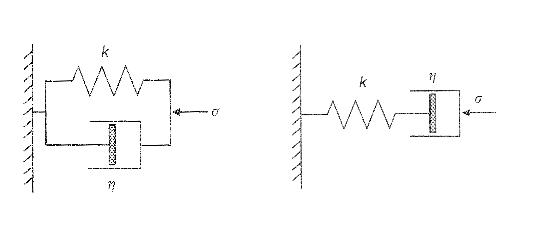
\includegraphics[width=0.95\textwidth]{figures/rheomod_vel.eps}
\caption{Mathematical modeling of reversible rate-dependent solid material behavior. Different combinations of a spring element with a
dashpot element \cite{JCZ:2007}: Kelvin-Voigt model (left) and Maxwell model (right)}
\label{fig:rheomod_vel}
\end{center}
\end{figure}

\newpage

The parallel connection of the spring and the dashpot elements is known as Kelvin-Voigt model. It is characterized by equal displacements
(and therefore equal strain values) in both of the individual elements, whereas the stress value of the model will be the sum of the
stresses in the spring and the dashpot. The constitutive behavior of the Kelvin-Voigt model is described by a differential equation.
\begin{equation}
\sigma\,=\,k\,\varepsilon\,+\,\eta\,\mathop{\varepsilon}\limits^{\miu{.}{}{}}
\label{eq:kelvin}
\end{equation}
If a stress $\sigma_0$ is instantaneously applied to a Kelvin-Voigt model, which is held constant thereafter, the solution of the
differential equation (\ref{eq:kelvin}) is given as follows:
\begin{equation}
\varepsilon\,=\,\frac{\sigma_0}{k}\,\left[1\,-\,\mathrm{e}^{-kt/\eta}\right]
\end{equation}
which indicates that the strain increases asymptotically to its steady-state (elastic) value $\sigma_0/k$. Thus, the Kelvin-Voigt model
represents the typical strain retardation, but neglecting any instantaneous strain.

The series connection of the spring and the dashpot elements is known as Maxwell model. Within this context, equal stress values occur in
both of the individual elements, whereas the total displacement (and therefore the strain) of the model will be the sum of the
displacements in the spring and the dashpot. The constitutive behavior of the Maxwell model can again be described by a differential
equation. 
\begin{equation}
\mathop{\varepsilon}\limits^{\miu{.}{}{}}\,=\,\frac{1}{\eta}\,\sigma\,+\,\frac{1}{k}\,\mathop{\sigma}\limits^{\miu{.}{}{}}
\label{eq:maxwell}
\end{equation}
Applying an instantaneous stress, a Maxwell element exhibits an instantaneous elastic response characterized by the spring constant $k$,
and a long-term viscous response specified by the viscosity $\eta$. If the Maxwell substance is subjected to an instantaneous jump in
strain with the amplitude $\varepsilon_0$, which is held constant thereafter, the differential equation (\ref{eq:maxwell}) can be solved closely.
The solution
\begin{equation}
\sigma\,=\,k\,\varepsilon_0\,\mathrm{e}^{-kt/\eta}
\end{equation}
indicates a stress decrease (relaxation) at constant (non-zero) strain, whereas in case of the Maxwell model the stress relaxes to zero,
simulating the behavior of a viscoelastic fluid.

\subsection{Viscoplasticity}
\label{sec:viscoplast}

Viscoplasticity is the most general material class, and the constitutive theories of viscoplasticity must be defined, on principle, to model all macroscopically observable phenomena of material behavior. The viscoplastic material class combines elements of all the other classes presented above. Micromechanical phenomena causing viscoplastic material behavior are exceptionally complex. 

Here, we will focus only on one typical effect of viscoplastic material behavior particularly relevant for geomaterials -- creep processes. Although in both cases characterizing the strain evolution at constant stress, viscoplastic creep differs from the viscoelastic creep (retardation) mentioned above, because no asymptotical strain value will be reached in the viscoplastic case. A typical viscoplastic creep curve is shown in Fig.~\ref{fig:creep}.

\begin{figure}[htb!]
\begin{center}
\footnotesize
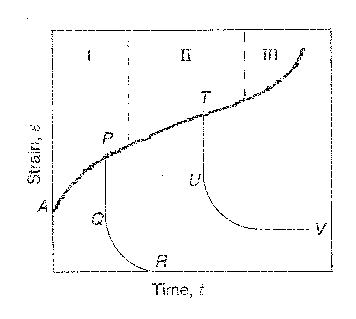
\includegraphics[width=0.5\textwidth]{figures/creep.eps}
\caption{Schematical representation of a viscoplastic creep curve showing the three typical periods: primary, secondary, and tertiary creep \cite{JCZ:2007}. The three periods are indicated by the Roman numerals I, II and III, the point $A$ indicates the instantaneous elastic strain}
\label{fig:creep}
\end{center}
\end{figure}

For the viscoplastic creep behavior, generally, three typical periods can be observed. Whereas at all creep periods strain increases without reaching any asymptotical value, they differ in the strain rate. The first period, called primary creep, is characterized by a decreasing creep rate (transient creep), while for the second creep period, called secondary creep, a constant strain rate is observed (stationary creep, steady-state creep). The period of more or less constant strain rate is followed by the tertiary creep with ever-inreasing strain rate, eventually causing mechanical failure of the structure under consideration. The total reduction of the applied stresses results in a strain relaxation. Unloading in the primary creep period is characterized by a complete strain relaxation (similar to viscoelatic behavior). However, if stress is removed during the secondary creep period, residual strains remain (effect of plasticity).

Comparable to theory of elastoplasticity, as starting point for the constitutive modeling of viscoplastic stress-strain states serves the functional relation between the stress rate and the elastic strain rate (\ref{eq:elplastmatlaw}). The overall strain tensor is additively decomposed into several constitutive parts: apart from the partial elastic and plastic strain tensors a creep strain tensor is introduced $\miu{\varepsilon}{\mathrm{c}}{}$.
\begin{equation}
\miu{\varepsilon}{}{\dot}\,=\,\miu{\varepsilon}{\mathrm{el}}{\dot}\,+\,\miu{\varepsilon}{\mathrm{pl}}{\dot}\,+\,\miu{\varepsilon}{\mathrm{c}}{\dot}
\label{eq:strainsplit_vpl}
\end{equation}
Similar to the plastic potential (yield condition), the creep behavior is mathematically characterized based on appropriately defined creep potentials $\Phi_{\mathrm{c}}(\miu{\sigma}{}{})$ representing, again, relationships among the coefficients of the stress tensor. Consequently, the creep strain rate tensor is defined as follows:
\begin{equation}
\miu{\varepsilon}{\mathrm{c}}{\dot}\,=\,
\lambda_{\mathrm{c}}\,\frac{\partial\Phi_{\mathrm{c}}(\miu{\sigma}{}{})}{\partial\miu{\sigma}{}{}}
\label{eq:creepstrainrate}
\end{equation}
with the so-called creep multiplier $\lambda_{\mathrm{c}}$. Consequently, the constitutive relation (\ref{eq:elplastmatlaw}) can be
reformulated. 
\begin{equation}
\miu{\sigma}{}{\dot}\,=\,\fourtens{C}
\left(\miu{\varepsilon}{}{\dot}\,-\,
\lambda_{\mathrm{pl}}\,\frac{\partial\Phi_{\mathrm{pl}}(\miu{\sigma}{}{})}{\partial\miu{\sigma}{}{}}
\,-\,
\lambda_{\mathrm{c}}\,\frac{\partial\Phi_{\mathrm{c}}(\miu{\sigma}{}{})}{\partial\miu{\sigma}{}{}}
\right)
\label{eq:vplastmatlawmod}
\end{equation}

In geomechanics, the long-term rock behavior during the stationary creep period is the main focus of interest. One widely-used creep potential characterizing secondary creep is the so-called Norton's model
\begin{equation}
\Phi_{\mathrm{c}}(\miu{\sigma}{}{})\,=\,
\frac{\alpha}{n+1}\,
\left(\sqrt{\ttfrac{3}{2}\miu{\sigma}{d}{}\ccdot\miu{\sigma}{d}{}}\right)^{n+1}
\label{eq:norton}
\end{equation}
with the material parameters $\alpha$ and $n$.

\vspace{4.0ex}
All of the constitutive models mentioned above are idealized approximations of the actual material behavior. The presented models are relatively simple, and allow to gain a first insight into the material theory of deformable solid substances. Some other aspects, which are relevant for rock mechanics analyzing material behavior could not be considered here, and are subject of further studies, like:
\begin{itemize}
\item Rate-dependent deformation processes in porous media are caused by the pore pressure diffusion through the solid skeleton at a finite rate, and intrinsic viscous properties of the matrix material. A separated experimental observation of theses effects is quite challenging with according consequences to the constitutive modeling.
\item Certain geomaterials show a layered structure (e.g. shale, sandstone). Consequently, material properties of these substances depend on the direction of the impact of external forces (known as anisotropic material behavior), which has to be considered in constitutive relations.
\item Damage and failure of rocks play an important role in real geoprocesses, and require an individual consideration.
\item The analysis of wave propagation (dynamic phenomena) in geomaterials is relevant for all kinds of seismic activities or seismic analyses.
\item The design of appropriate lab tests is essential for the fundamental characterization of the material behavior, and the calibration of constitutive models.
\end{itemize}
